\documentclass[12pt,a4paper]{article}

% Paquetes de configuración del documento
\usepackage[utf8]{inputenc}
\usepackage[spanish]{babel}
\usepackage[T1]{fontenc}
\usepackage[margin=2.5cm]{geometry}
\usepackage{fancyhdr}
%Paquetes para simbologia%
\usepackage{amsmath}
\usepackage{amsfonts}
\usepackage{amssymb}
\usepackage{physics}
\usepackage{longtable}
\usepackage{graphicx}
\usepackage{caption}
\usepackage{float}
\usepackage{xurl}
\usepackage[colorlinks=true,
            linkcolor=black,
            urlcolor=myblue,
            citecolor=black,
            filecolor=black]{hyperref}
 % Opción estándar para enlaces
\Urlmuskip=0mu plus 1mu          % Mejora el espaciado para permitir cortes
\usepackage{subcaption}  % en el preámbulo
\usepackage{pgfplots}
\usepackage{pdfpages}
\pgfplotsset{compat=1.18}
\usepackage{tikz}
\usepackage{xcolor}
\definecolor{myblue}{RGB}{42, 127, 179}

% Encabezado
\pagestyle{fancy}
\lhead{\textit{Ingeniería Mecánica}}
\chead{\textit{Materiales Metálicos}}
\rhead{\textit{UTN-FRVM}}

\begin{document}
\begin{titlepage}
	
	\begin{center}
		{\huge \textit{Universidad Tecnológica Nacional}}\\
        \vspace{0.5cm}
		{\LARGE \textit{Facultad Regional Villa María}}\\
		\vspace{1.5cm}
        {\LARGE{\textit{Ingeniería Mecánica - Materiales Metálicos}}}\\
		\vspace{1.5cm}
        \LARGE{\textit{Trabajo Práctico 3-06}}
	\end{center}
	
	\vfill

    \textit{Grupo DEL RÍO:}
	\begin{itemize}
		\item \textit{Abregú, Iván.}
		\item \textit{Antico, Rodrigo.}
		\item \textit{Brussa,Julián.}
		\item \textit{Cabral, Franco.}
        \item \textit{Cárdenas, Felipe.}
        \item \textit{Cardozo, Martín.}
        \item \textit{Córdoba, Nathan.}
        \item \textit{Cucco, Ramiro.}
        \item \textit{del Río, Juan.}
        \item \textit{Guerini, Nazareno.}
        \item \textit{Medina, Ivo.}
        \item \textit{Ortiz, Gastón.}
        \item \textit{Picos, Elías.}
        \item \textit{Quinteros, Lautaro.}
	\end{itemize}
    
	\textit{Docentes:}
	\begin{itemize}
		\item \textit{Dr. Lucioni, Eldo José.}
		\item \textit{Ing. Victorio Vallaro, Juan Manuel.}
	\end{itemize}
	\centering
	\today
	
\end{titlepage}

\tableofcontents
\begin{abstract}
    \underline{\textbf{Requerimiento del Trabajo.}}
    Analice e investigue el contenido del catálogo que se indica a fin de adquirir la capacidad de explicar el significado de la información que allí se detalla:
    \begin{itemize}
        \item Böhler. Centro de Materiales. Sitio Web: \url{https://www.acerosboehler.com.ar/es/material-center/}
        \item Böhler. Catálogo de aceros para herramientas. \url{https://www.acerosbohler.com/app/uploads/sites/101/2019/08/B%C3%B6hler_toolsteel_2018_LQ.pdf}
        \item Arcelor-Mittal. Catálogo de Productos. Sitio Web: \url{https://www.acindar.com.ar/wp-content/uploads/2018/11/Catalogode-productos-para-la-industria.pdf}
        \item IRAM - Hojas Características de los Aceros \{MM-CAD-TP 2-01\}
        \item SSAB. Su guía para los productos de acero antidesgaste Hardox\textsuperscript{\textregistered}. Sitio Web: \url{https://www.ssab.lat/marcas-y-productos/hardox/productprogram}
    \end{itemize}
\end{abstract}

\section{Análisis Aceros Böhler.}
Son aceros producidos por Böhler, uno de los líderes internacionales de aceros para herramientas, aceros rápidos y aceros especiales. También se los suele clasificar por su ruta de fundición en aceros convencionales, refundidos por electroescoria (ESR/ESU), pulvimetalúrgicos de tercera generación y aceros atomizados en polvo para fabricación aditiva.

Se solicita una descripción del catálogo, que se realiza a continuación:

\subsection{Designaciones.}
Estos productos están catalogados como \textbf{Böhler Xxxx} donde la “X” es una letra que da una cierta clasificación, seguida por tres dígitos “xxx”. Algunas de las designaciones más importantes son:

\begin{itemize}
    \item \textbf{S}: Aceros rápidos, que pueden ser:
    \begin{itemize}
        \item Aceros rápidos convencionales.
        \item Aceros rápidos refundidos por electroescoria (ESR).
        \item Aceros rápidos pulvimetalúrgicos.
    \end{itemize}
        \begin{figure}[H]    
        \centering         
        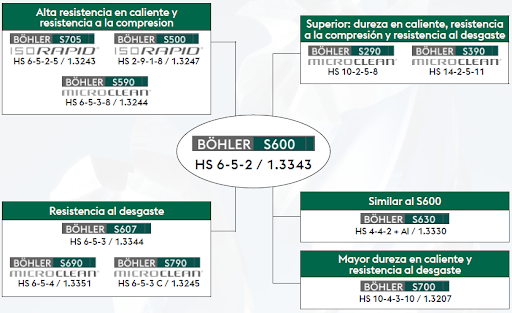
\includegraphics[width=0.85\linewidth]{Inagenes para latex/1.png}
    \end{figure}
    \item \textbf{K}: Aceros para trabajo en frío, que pueden ser:
    \begin{itemize}
        \item Aceros para trabajo en frío convencionales.
        \item Aceros para trabajo en frío refundidos por electroescoria (ESR).
        \item Aceros para trabajo en frío pulvimetalúrgicos.
    \end{itemize}
    \begin{figure}[H]    
        \centering         
        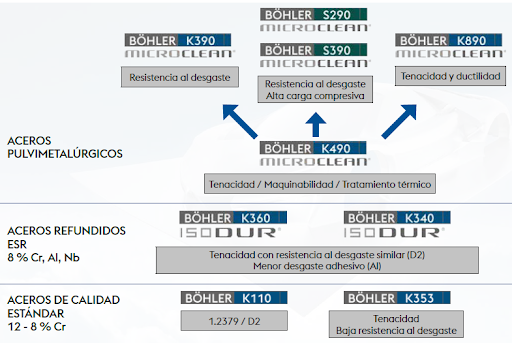
\includegraphics[width=0.85\textwidth]{Inagenes para latex/2.png}
    \end{figure}
    \item \textbf{N}: Aceros para cuchillas.
    \begin{figure}[H]    
        \centering         
        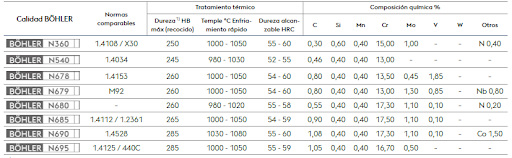
\includegraphics[width=0.9\textwidth]{Inagenes para latex/3.png}
    \end{figure}
    \item \textbf{W}: Aceros para trabajo en caliente, que se clasifican en:
    \begin{itemize}
        \item Aceros para trabajo en caliente convencionales con tratamiento térmico especial.
        \item Aceros para trabajo en caliente refundidos por electroescoria (ESR).
        \item Aceros para trabajo en caliente fundidos en vacío (VAR).
    \end{itemize}
    \begin{figure}[H]    
        \centering         
        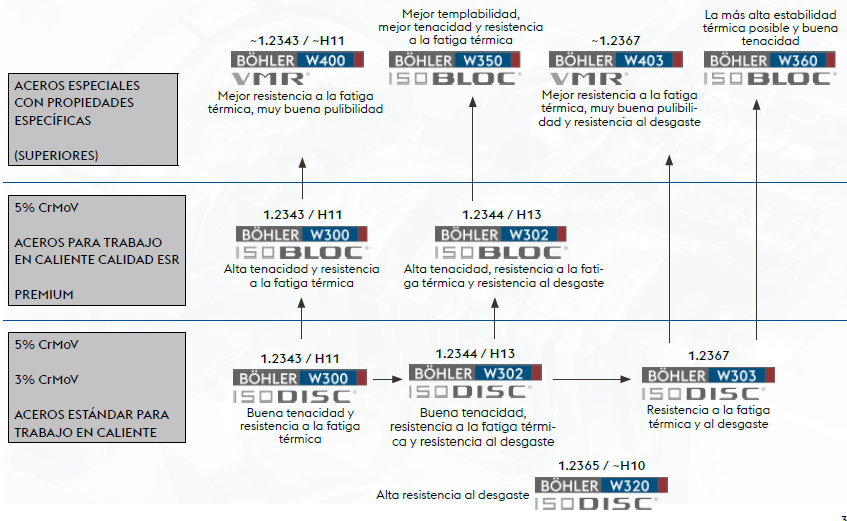
\includegraphics[width=0.6\textwidth]{Inagenes para latex/4.png}
    \end{figure}
    \item \textbf{M}: Aceros para moldes de plástico:
    \begin{itemize}
        \item Aceros para moldes de plástico convencionales.
        \item Aceros para moldes de plástico con características especiales.
        \item Aceros para moldes de plástico con resistencia al desgaste.
        \item Aceros para moldes de plástico fundidos en vacío (VAR).
        \item Aceros para moldes de plástico refundidos por electroescoria (ESR).
        \item Aceros para moldes de plástico pulvimetalúrgicos.
    \end{itemize}
    \begin{figure}[H]    
        \centering         
        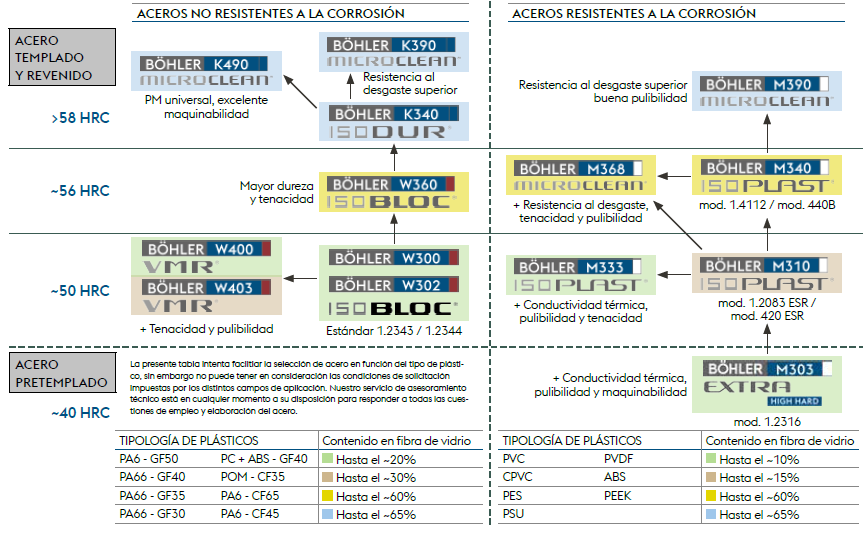
\includegraphics[width=0.8\textwidth]{Inagenes para latex/5.png}
    \end{figure}
    \item \textbf{L}: Aceros para fabricación aditiva (atomizados en polvo).
\end{itemize}
\begin{figure}[H]    
    \centering         
    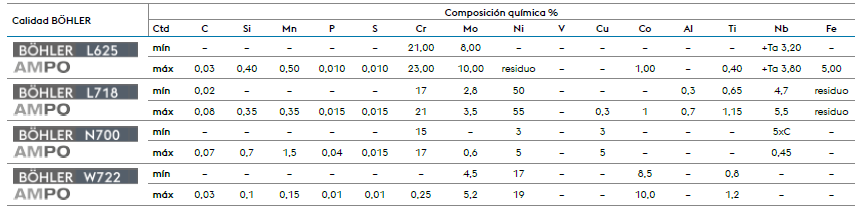
\includegraphics[width=0.8\textwidth]{Inagenes para latex/6.png}
\end{figure}

Además, se nombran las aplicaciones y sectores para los cuales se emplean estos aceros: \textit{automoción, aeronáutica, aeroespacial, bienes de consumo, herramientas de corte, oil y gas, y sector energético}, entre otros.

\subsection{Rutas de producción.}
\textbf{Producción convencional.} Menor rendimiento en comparación con calidades ESR\footnote{\textit{Electroslag.}} y PM (Producción pulvimetalúrgica) debido a:
\begin{itemize}
    \item Distribución desigual de los carburos.
    \item Cierto grado de segregaciones.
    \item Bajo nivel de homogeneidad.
    \item Bandas de carburos marcadas, sobre todo en el núcleo de piezas grandes.
    \item Cierta variedad en el tamaño de los carburos.
    \item \textit{Estabilidad dimensional} desigual en sentidos longitudinal y transversal.
\end{itemize}
\begin{figure}[H]    
    \centering         
    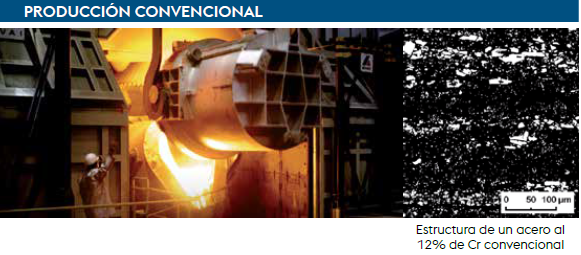
\includegraphics[width=0.75\textwidth]{Inagenes para latex/7.png}
\end{figure}
\textbf{Producción ESR/ESU.} Vida útil más larga gracias a:
\begin{itemize}
    \item Mínimas inclusiones no metálicas.
    \item Menos micro/macro segregaciones.
    \item Buena homogeneidad y alta pureza.
    \item Estructura homogénea en toda la sección y longitud de la barra.
    \item Distribución uniforme de los carburos en barras de grandes dimensiones.
    \item Estabilidad dimensional.
    \item Amplia gama de aplicaciones gracias a altos niveles de resistencia.
\end{itemize}

\begin{figure}[H]
    \centering
    \begin{subfigure}{0.45\textwidth}
        \centering
        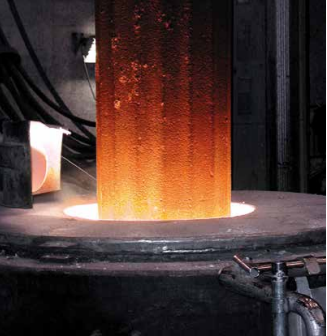
\includegraphics[width=\textwidth]{Inagenes para latex/8 izq.png}
    \end{subfigure}
    \begin{subfigure}{0.45\textwidth}
        \centering
        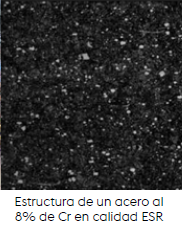
\includegraphics[width=\textwidth]{Inagenes para latex/8 der.png}
    \end{subfigure}
\end{figure}

\textbf{Producción pulvimetalúrgica (PM).} Para máximas exigencias:
\begin{itemize}
    \item Óptima distribución de carburos.
    \item Máxima pureza metalúrgica.
    \item Acero libre de segregaciones.
    \item Propiedades isotrópicas.
    \item Máxima resistencia al desgaste y gran tenacidad.
    \item Alta dureza.
    \item Muy buena estabilidad dimensional.
    \item Elevada resistencia a la presión.
    \item Buena pulibilidad.
\end{itemize}
\begin{figure}[H]    
    \centering         
    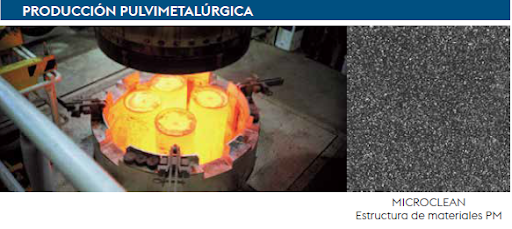
\includegraphics[width=0.85\textwidth]{Inagenes para latex/9.png}
\end{figure}

\subsection{Equivalencias de designaciones.}
Por último, en el catálogo se aprecia la equivalencia del acero Böhler con otros sistemas de nomenclatura:

\begin{itemize}
    \item Nomenclatura EN (Sistema Europeo).
    \item Nomenclatura UNS (Sistema Unificado de Numeración).
    \item Nomenclatura ASTM.
    \item Nomenclatura SAE/AISI.
    \item Nomenclatura JIS (Sistema Japonés).
\end{itemize}

\begin{table}[h!]
    \centering
    \begin{tabular}{llll}
        \hline
        \textbf{BÖHLER} & \textbf{EN} & \textbf{JIS} & \textbf{AISI} \\ \hline
        S601 & HS6-5-2 & SKH51 & M2 \\ \hline
    \end{tabular}
    \caption{Ejemplo de equivalencias extraído del catálogo.}
    \label{tab:equivalencias-bohler}
\end{table}

\section{Análisis ArcelorMittal.}
Es una compañía siderúrgica productora de aceros largos que abastece a los sectores de la construcción civil, agro e industria en general.

\subsection{Sector Agro.}
En este sector se fabrican postes, alambres, esquineros y varillas que reemplazan totalmente otros materiales, como la madera.

\paragraph{Alambres.}
Alambres ovalados galvanizados; Alambres redondos galvanizados; Trenza galvanizada; Alambre de púas; Alambre para riendas y maneas; Tejidos galvanizados; entre otros.

\paragraph{Postes.}
Poste esquinero de acero; Poste intermedio facón.

\paragraph{Varillas.}
Varillas de alambre galvanizado; Varillas T.

Cada producto cuenta con su respectiva tabla de especificaciones técnicas. algunos ejemplos a continuación.
\begin{figure}[H]    
    \centering         
    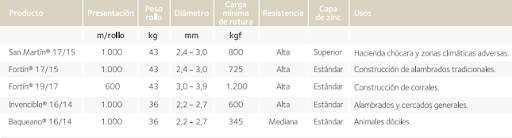
\includegraphics[width=1\textwidth]{Inagenes para latex/10.png}
    \caption*{*Alambres ovalados galvanizados}
\end{figure}
 \begin{figure}[H]    
    \centering         
    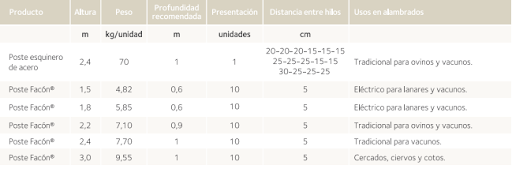
\includegraphics[width=1\textwidth]{Inagenes para latex/11.png}
    \caption*{*Tabla de Postes}
\end{figure}
 \begin{figure}[H]    
    \centering         
    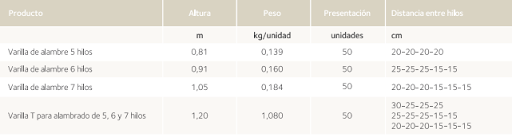
\includegraphics[width=1\textwidth]{Inagenes para latex/12.png}
    \caption*{*Tabla de Varillas}
\end{figure}


\subsection{Construcciones Civiles.}
Los productos que se ofrecen para este sector son:

\begin{itemize}
    \item DN A 420\textsuperscript{\textregistered} Barras de acero de dureza natural para hormigón armado.
    \item AL 220\textsuperscript{\textregistered} Barras de acero lisas para hormigón armado.
    \item Soluciones Acindar: Acero cortado y doblado.
    \item Sima\textsuperscript{\textregistered} Mallas soldadas estándar.
    \item Sima\textsuperscript{\textregistered} Mallas soldadas según especificación.
    \item Soluciones Acindar: Estructuras prearmadas de acero.
    \item Trilogic\textsuperscript{\textregistered} Vigas reticuladas electrosoldadas de acero.
    \item Clavos.
    \item Job-Shop: Mallas electrosoldadas para uso no estructural.
    \item Tejimet\textsuperscript{\textregistered}: Alambres tejidos galvanizados.
    \item Perfiles laminados en caliente (ángulo de alas iguales, perfil normal U, perfil normal doble T, perfil IPB, IPBL, IPE, U y T chicos).
    \item Barras laminadas en caliente.
    \item Planchuelas laminadas.
    \item Alambre recocido.
    \item Alambres de acero para pretensado.
    \item Cordones de acero para pretensado.
    \item Cordón engrasado envainado.
\end{itemize}

Cada producto consta de su respectiva hoja técnica, a continuación pondremos algunas como referencia:

 \begin{figure}[H]    
    \centering         
    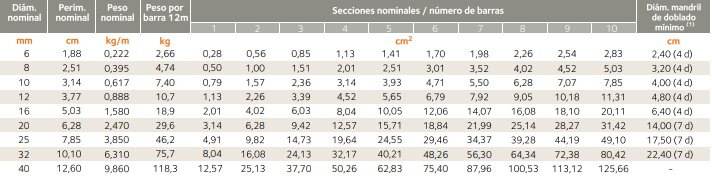
\includegraphics[width=1\textwidth]{Inagenes para latex/13.png}
    \caption*{*Tabla Con Especificsciones de las Barras  DN A 420\textsuperscript{\textregistered}}
\end{figure}
\begin{figure}[H]    
    \centering         
    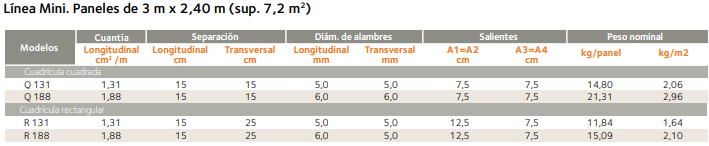
\includegraphics[width=1\textwidth]{Inagenes para latex/14.png}
    \caption*{*Tabla Con Especificaciones de Malla}
\end{figure}
\begin{figure}[H]
    \centering
    \begin{minipage}{0.45\textwidth}
        \centering
        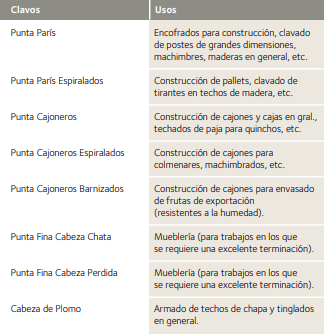
\includegraphics[width=\textwidth]{Inagenes para latex/15 izq.png}
    \end{minipage}
    \begin{minipage}{0.45\textwidth}
        \centering
        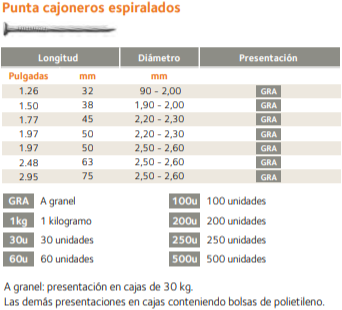
\includegraphics[width=\textwidth]{Inagenes para latex/15 der.png}
    \end{minipage}
    \caption*{*Algunas tablas de especificaciones sobre Clavos}
\end{figure}

\subsection{Productos para la Industria.}
Los productos del catálogo para este sector son:
\begin{itemize}
    \item Palanquillas de colada continua.
    \item Barras laminadas uso mecánico.
    \item Barras laminadas apto forja.
    \item Barras trefiladas.
    \item Barras laminadas y trefiladas para resortes.
    \item Barras rectificadas.
    \item Planchuelas para elásticos.
\end{itemize}

\begin{figure}[H]    
    \centering         
    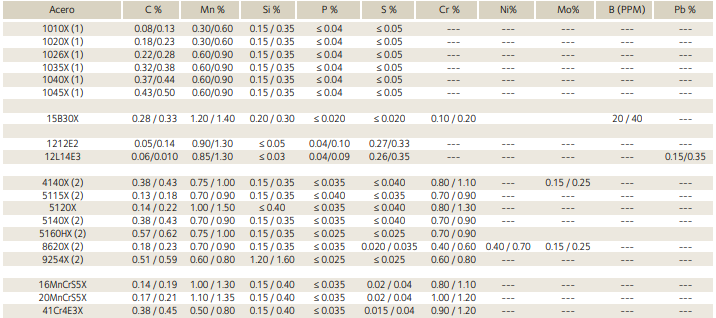
\includegraphics[width=1\textwidth]{Inagenes para latex/16.png}
    \caption*{*Tabla de referencia de los tipos de aceros que son utilizados para diferentes productos}
\end{figure}
\begin{figure}[H]    
    \centering         
    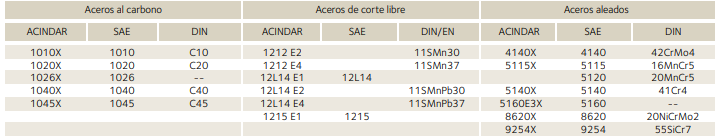
\includegraphics[width=1\textwidth]{Inagenes para latex/17.png}
    \caption*{*Tabla de equivalencias con las distintas normas}
\end{figure}
\begin{figure}[H]
    \centering
    \begin{minipage}{0.45\textwidth}
        \centering
        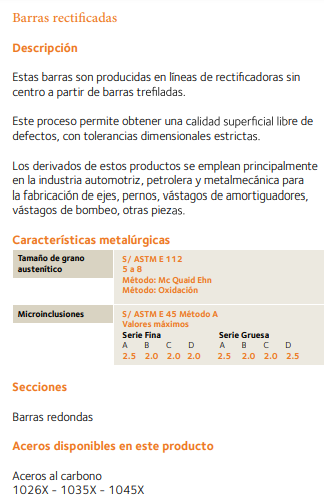
\includegraphics[width=\textwidth]{Inagenes para latex/18.png}
    \end{minipage}
    \begin{minipage}{0.45\textwidth}
        \centering
        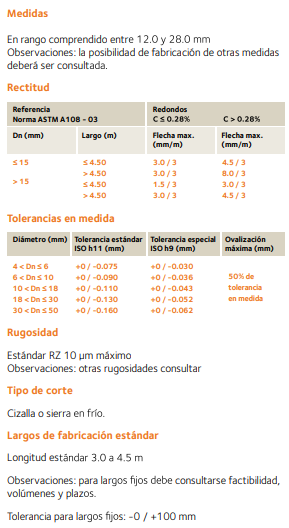
\includegraphics[width=\textwidth]{Inagenes para latex/19.png}
    \end{minipage}
    \caption*{*Ejemplo de las descripciones mencionadas de cada producto de carácter industrial}
\end{figure}

\section{Hojas Características IRAM.}
La clasificación de los aceros IRAM en el archivo adjunto se organiza en 4 grupos:
\begin{itemize}
    \item Aceros al carbono.
    \item Aceros de corte libre.
    \item Aceros de alto manganeso.
    \item Aceros aleados.
\end{itemize}

Cada designación tiene un enlace asociado que lleva a la respectiva ficha técnica del acero.
A continuación un ejeplo de de estas hojas técnicas:

\paragraph{Ejemplo}
Acero al Carbono 1060. Se puede ver la hoja técnica de este acero en el \hyperref[anexo]{anexo}

\section{Análisis SSAB.}
Empresa que vende productos manufacturados de aceros de gran calidad y resistencia. Divide sus productos en:
\begin{itemize}
    \item \textbf{Strenx\textsuperscript{\textregistered}.}
    \item \textbf{Hardox\textsuperscript{\textregistered}.}
    \item \textbf{Toolox\textsuperscript{\textregistered}.}
    \item \textbf{Armox\textsuperscript{\textregistered}.}
    \item \textbf{Duroxite\textsuperscript{\textregistered}.}
    \item \textbf{SSAB Docol\textsuperscript{\textregistered}.}
\end{itemize}

\subsection{Hardox\textsuperscript{\textregistered} $\Rightarrow$ Aceros antidesgaste}
En este trabajo nos centraremos en los aceros Hardox\textsuperscript{\textregistered} debido a que el  requerimiento de la actividad nos indica específicamente tratar sobre estos aceros.
La chapa antidesgaste Hardox\textsuperscript{\textregistered} está disponible en numerosas calidades para satisfacer exigencias de aplicaciones resistentes al desgaste, desde equipos de minería y construcción hasta el transporte pesado.

\begin{figure}[H]    
    \centering         
    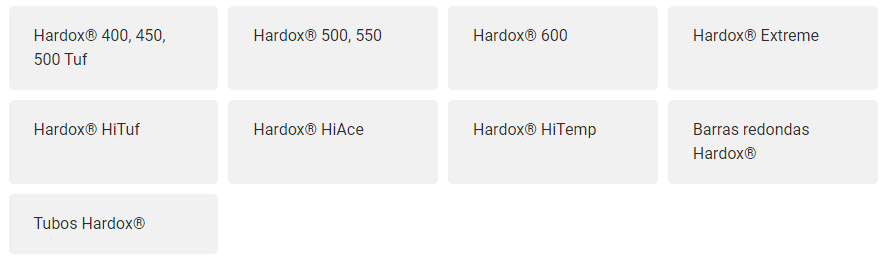
\includegraphics[width=1\textwidth]{Inagenes para latex/25.png}
    \caption*{*Estos son los aceros Hardox\textsuperscript{\textregistered} antidesgaste que ofrece SSAB}
\end{figure}
\paragraph{SSAB Concretamente Divide y Describe los Distintos Tipos de Aceros Antidesgaste de la Siguiente Forma, de Acuerdo al Uso Que Tengan:}

\begin{enumerate}
    \item Primero hace una breve descricpción de los aceros que estén agrupados dentro de un tipo de uso.
    \item Después de la descripción, nos muestran una tabla con los datos más importantes que son: nombre del produco, rango de espesores, dureza (puede estar en diferentes denominaciones), en algunos esta el CET (CEV) típico que es un parámetro metalúrgico que describe la soldabilidad del acero y su tendencia a formar estructuras duras y frágiles (martensita) en la zona afectada por el calor (ZAC) durante la soldadura, y también en algunos nos muestran la energía de impacto garantizada para ensayos transversales/energía de impacto típica para ensayos longitudinales.
    \item A la derecha, en la última columna, todas las tablas tienen el simbolo de descarga para poder descargar una ficha técnica con más detalles de un acero en particular.
\end{enumerate}

\begin{itemize}
    \item \textbf{Aceros antidesgaste con propiedades estructurales Hardox\textsuperscript{\textregistered} 400, Hardox\textsuperscript{\textregistered} 450 y Hardox\textsuperscript{\textregistered} 500 Tuf.}
    \begin{figure}[H]    
        \centering         
        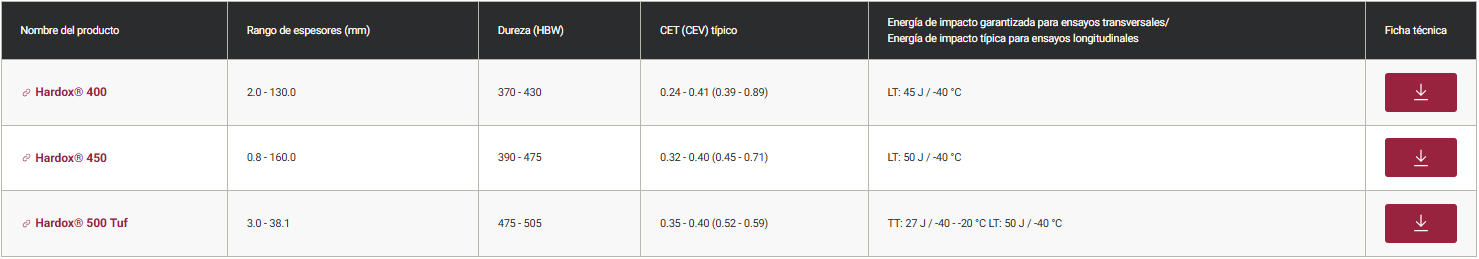
\includegraphics[width=1\textwidth]{Inagenes para latex/26.png}
    \end{figure}
    \item \textbf{Aceros Hardox\textsuperscript{\textregistered} 500 y Hardox\textsuperscript{\textregistered} 550 para condiciones de desgaste difíciles.}
    \begin{figure}[H]    
        \centering         
        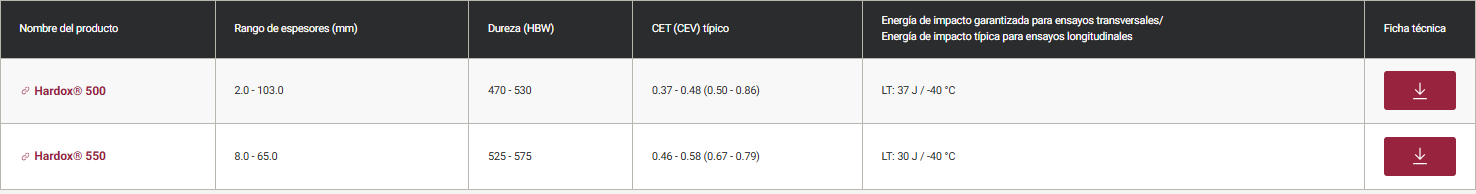
\includegraphics[width=1\textwidth]{Inagenes para latex/27.png}
    \end{figure}
    \item \textbf{El acero Hardox\textsuperscript{\textregistered} 600 ofrece una resistencia superior al desgaste.}
    \begin{figure}[H]    
        \centering         
        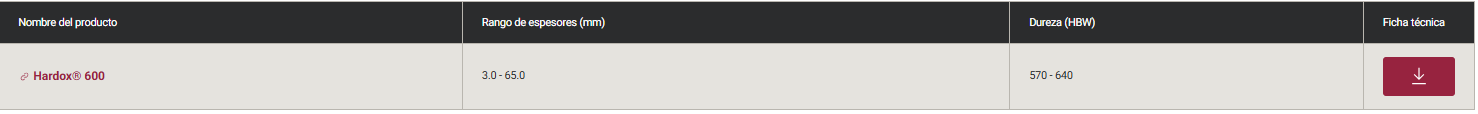
\includegraphics[width=1\textwidth]{Inagenes para latex/28.png}
    \end{figure}
    \item \textbf{El acero Hardox\textsuperscript{\textregistered} Extreme ofrece una resistencia al desgaste radical.}
    \begin{figure}[H]    
        \centering         
        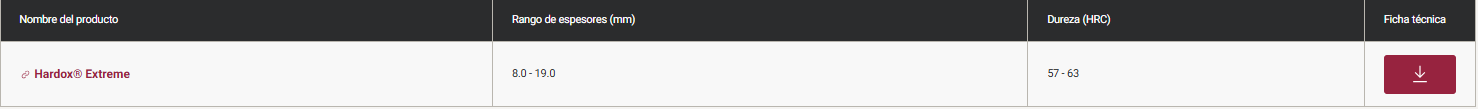
\includegraphics[width=1\textwidth]{Inagenes para latex/29.png}
    \end{figure}
    \item \textbf{Acero Hardox\textsuperscript{\textregistered} HiTuf para las aplicaciones de desgaste estructural más gruesas.}
    \begin{figure}[H]    
        \centering         
        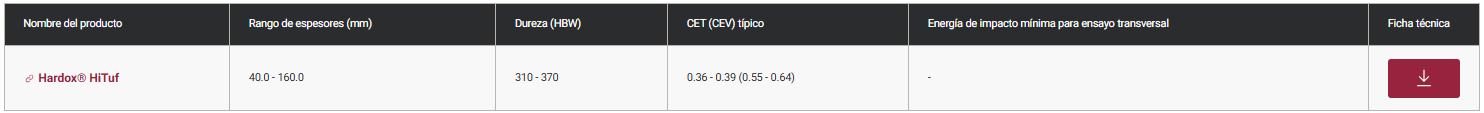
\includegraphics[width=1\textwidth]{Inagenes para latex/30.png}
    \end{figure}
    \item \textbf{Acero Hardox\textsuperscript{\textregistered} HiAce resistente al desgaste en entornos ácidos.}
    \begin{figure}[H]    
        \centering         
        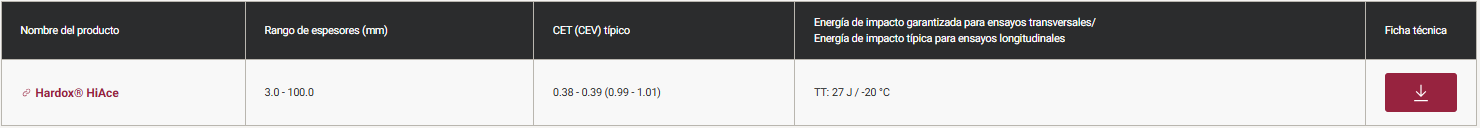
\includegraphics[width=1\textwidth]{Inagenes para latex/31.png}
    \end{figure}
    \item \textbf{Acero Hardox\textsuperscript{\textregistered} HiTemp resistente al desgaste a temperaturas elevadas.}
    \begin{figure}[H]    
        \centering         
        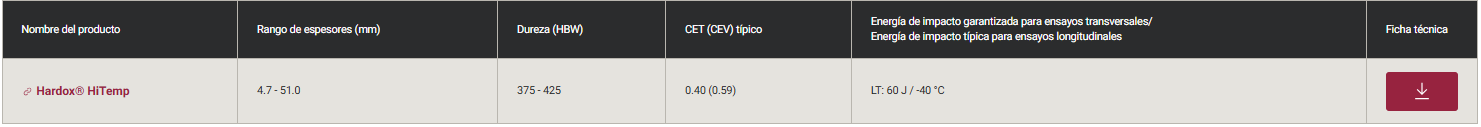
\includegraphics[width=1\textwidth]{Inagenes para latex/32.png}
    \end{figure}
    \item \textbf{Barras redondas de Hardox\textsuperscript{\textregistered}.}
    \begin{figure}[H]    
        \centering         
        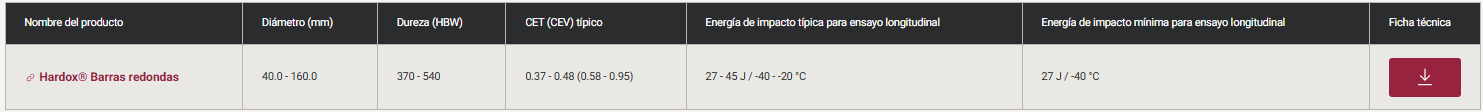
\includegraphics[width=1\textwidth]{Inagenes para latex/33.png}
    \end{figure}
    \item \textbf{Tubos de acero Hardox\textsuperscript{\textregistered}.}
    \begin{figure}[H]    
        \centering         
        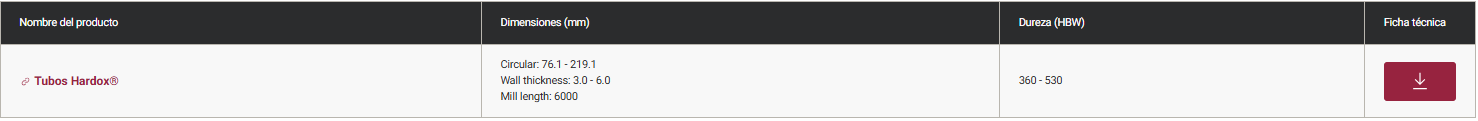
\includegraphics[width=1\textwidth]{Inagenes para latex/34.png}
    \end{figure}
\end{itemize}

\textbf{Ejemplo:} Haremos un ejemplo con el acero  Hardox\textsuperscript{\textregistered} 400 de aceros antidesgaste con propiedades estructurales. Con una dureza nominal de 400 HBW, el acero Hardox\textsuperscript{\textregistered} 400 es versátil y resistente a la abrasión. Además, es adecuado en aplicaciones de desgaste moderado que requieren una alta resistencia a impactos, una óptima capacidad de plegado y una excelente soldabilidad. En el anexo se puede ver la ficha técnica.

\section{Bibliografía.}
\begin{itemize}
    \item \url{https://www.acerosbohler.com/app/uploads/sites/101/2023/01/BOH_018_Acero_para_plasticos_reforzados.pdf}
    \item \url{https://www.acerosbohler.com/app/uploads/sites/101/2019/08/B%C3%B6hler_toolsteel_2018_LQ.pdf}
    \item \url{https://www.acerosboehler.com.ar/es/material-center/}
    \item \url{https://www.acindar.com.ar/wp-content/uploads/2018/11/CatalogoAgro.pdf}
    \item \url{https://www.acindar.com.ar/wp-content/uploads/2020/09/Catalogo_Construccion_civil.pdf}
    \item \url{https://www.acindar.com.ar/wp-content/uploads/2018/11/Catalogo-de-productos-para-la-industria.pdf}
    \item \url{https://www.ssab.com/es-mx/marcas-y-productos/hardox/programa-de-producto}
\end{itemize}

\vfill
\textit{\textbf{Este trabajo fue elaborado con la ayuda de la IA para facilitar la confección y disposición de los elementos en dicho trabajo; y la búsqueda de información para complementar la dada por la cátedra.}}
\appendix
\section{Hojas técnicas de ejemplo.}

\clearpage
\thispagestyle{empty}  
\includepdf[
  pages=1,
  pagecommand={
    \begin{tikzpicture}[remember picture,overlay]
      \node at (current page.north) [yshift=-3.3cm] 
        {\Huge\bfseries Hoja técnica 1060 IRAM};
    \end{tikzpicture}
  }
]{1060.pdf}\label{anexo}
\includepdf[pages={2,5}]{1060.pdf}

\clearpage
\thispagestyle{empty}  
\includepdf[
  pages=8,
  pagecommand={
    \begin{tikzpicture}[remember picture,overlay]
      \node at (current page.north) [yshift=-5cm] 
        {\Huge\bfseries Hoja técnica de algunos aceros BOHLER};
    \end{tikzpicture}
  }
]{BOHLER.pdf}
\includepdf[pages=9]{BOHLER.pdf}

\clearpage
\thispagestyle{empty}
\includepdf[
  pages=1,
  pagecommand={
    \begin{tikzpicture}[remember picture,overlay]
      \node at (current page.north) [yshift=-2.8cm] 
        {\Huge\bfseries Hoja técnica de Hardox\textsuperscript{\textregistered} 400};
    \end{tikzpicture}
  }
]{HARDOX.pdf} 
\includepdf[pages=2]{HARDOX.pdf}
\end{document}

